\documentclass[]{final_report}
\usepackage{graphicx}
\usepackage{hyperref}
\usepackage{listings}



%%%%%%%%%%%%%%%%%%%%%%
%%% Input project details
\def\studentname{Ciaran Palmer}
\def\projecttitle{SensorML on SenseTile}
\def\supervisorname{Dr. Joseph Kiniry}
\def\moderatorname{-}


\begin{document}

\maketitle
\tableofcontents\pdfbookmark[0]{Table of Contents}{toc}\newpage

%%%%%%%%%%%%%%%%%%%%%%
%%% Your Abstract here

\begin{abstract}
This thesis evaluates the Sensor Model Language(SensorML) and Sensor Observation Service(SOS) specifications. These specifications are intended for use in the development of open sensor systems. The UCD CASL SenseTile sensor system is used as a case study for this evaluation. A SensorML model of SenseTile is developed. A SenseTile Web Service is also developed based on the SenseTile SensorML model and the SOS specification. This Web Service provides access to SenseTile sensor metadata and sensor observations. The thesis finally examines formalizing SensorML using a formal specification language called Business Object Notation.

\end{abstract}




\newpage


%%%%%%%%%%%%%%%%%%%%%%
%%% Acknowledgments

\chapter*{Acknowledgments}

Vieri del Bianco , Dragan Stosic and Joseph R. Kiniry.

%%%%%%%%%%%%%%%%%%%%%%
%%% Introduction

\chapter{Introduction}

Sensor systems are increasingly deployed to provide sensing information for a myriad of applications. These sensor systems contain many different sensor types and are developed by communities working in different domains. The heterogeneity of these systems means that interoperability is difficult and expensive. Reliably processing sensor observations retrieved from these heterogeneous systems is also problematic. Standard ways to describe sensors and to retrieve sensor data are needed to address the problem of sensor system heterogeneity. 

Standards are being developed to address the above issues. Two such standards are the Sensor Model Language (SensorML) specification\cite{SMLref} and the Sensor Observation Service (SOS) specification\cite{SOSref}. SensorML is a proposed standard for both describing sensors and describing the processing of sensor observations. The SOS specification is a proposed standard for retrieving sensor descriptions and sensor observations using Web Services. 

The SensorML and SOS specifications are developed by the Open Geospatial Consortium (OGC) as part of the Sensor Web Enablement (SWE) initiative \footnote{http://www.opengeospatial.org/projects/groups/sensorweb}. The members of the OGC have the goal of improving interoperability of sensor systems by developing open standards such as the SensorML and SOS specifications. This thesis investigates the use of these SWE SensorML and SOS standards in developing sensor systems.

A real sensor system called SenseTile[ref] is used as a case study for the evaluation of SensorML and SOS specifications. SenseTile is a sensor and processing package that contains motion sensors, temperature sensors, audio sensors, pressure sensors and light level sensors among others. It is a replacement for standard ceiling tiles to provide smart building services as part of a Web Sensor Network.

This thesis describes a  SensorML model of SenseTile, in particular the SenseTile Sensor Board. Based on this model a SenseTile Web Service prototype is developed to allow the retrieval of the SenseTile sensor descriptions and sensor observations. The Web Service is based on the SOS specification. An assessment of SensorML and SOS specifications is provided based on this work.

Currently there is no widely available formal definition of sensors or sensor data processing. Formal sensor descriptions allows sensor system development to use a formal verification based process. A verification based software development processes is described in \cite{Kiniryref} which has the goal of developing very robust software systems. Business Object Notatation(BON)\cite{BONref} is used in this process to formally specify the system being developed. BON is a notation and a method for analysis and design of Object Oriented systems. This thesis looks at how BON can be used to formally specify SensorML. The BON to SensorML mapping described in thesis allows SensorML sensor descriptions to then be refined to JML\footnote{http://www.eecs.ucf.edu/~leavens/JML/} and then to Java\footnote{http://www.java.com/}, as described in \cite{Kiniryref}.


\chapter{ Background Research}

\section{Sensor Web Enablement}\label{SWESec}
As described in the introduction the SensorML and SOS specifications are developed by the Open Geospatial Consortium (OGC) as part of the Sensor Web Enablement (SWE) initiative \footnote{http://www.opengeospatial.org/projects/groups/sensorweb}. The initiative is establishing interfaces and protocols to enable a standardized Sensor Web. This allows for easier integration of sensor applications across sensor systems. SWE provides a framework of open standards for use with Web-connected sensors and sensor systems. There are seven main specifications currently:

\begin{itemize}
\item  SensorModel Language(SensorML) - models and schema for sensor system description and sensor measurement processing
\item  Sensor Observation Service (SOS) - standard web interface for accessing sensor observations
\item  Observations \& Measurements (O\&M) - models and schema for packaging sensor observation values
\item  Transducer Markup Language (TML) - models and schema for multiplexed data from sensor systems
\item  Sensor Planning Service (SPS) - standard web interface for tasking sensor systems
\item  Sensor Alert Service (SAS) - standard web interface for publishing and subscribing to sensor alerts
\item  Web Notification Service (WNS) - standard web interface for asynchronous notification
\end{itemize}

SWE services based on the above specifications allow the discovery of sensors, access to the sensor data, as well as subscription to alerts, and tasking of sensors to control sensor meaurement. For a good overview of SWE and it's use in Sensor Web Networks see \cite{SWEArchref}.  The SensorML and SOS specifications, as mentioned, are used to develop the SenseTile Web Service. The O\&M specification is also used in developing the SenseTile Web Service. This specification defines the encoding of sensor observations and is used by the SOS specification. 


\section{Sensor Model Language}\label{SMLsection}
Sensor Modeling Language (SensorML) is primarily used to describe sensor systems and the processing of observations from sensor systems. The SensorML specification\cite{SMLref} provides a functional model of sensors and an XML encoding to describe sensors and their observations. Some of the main uses of SensorML described in the specification are:
\begin{itemize}
\item Support sensor and sensor observation discovery.
\item Support processing of the sensor observations.
\item Support geolocation information about sensors.
\item Provide accuracy information of sensors measurements.
\item Provide an executable process chain for deriving new data on demand.
\end{itemize}

XML Schema is used to specify the XML encoding of SensorML in the SensorML specification. This XML schema is based on two conceptual UML\footnote{http://www.uml.org/} models, the SensorML Conceptual Model and the SWE Common Conceptual Model, that describe SensorML. These models are explained in the following sections.

\subsection{SensorML Conceptual Model}
In SensorML sensors are modeled as processes that convert physical phenomena to data. Processes take inputs, process them and result in one or several outputs. For example, a process can take a measurement generated by a thermistor which might be an electrical resistance value and transform it to a Celsius value. Processes can also be connected together in process chains to allow the sensor data to be processed by several processes sequentially. These processes and process chains are modeled in SensorML as shown in the  below SensorML Conceptual Model \ref{fig:SMLConceptualModel}.

\begin{figure}[h]
\centering
\framebox{\scalebox{0.62}{\includegraphics{SMLConceptualModel.png}}}
\caption{SensorML Conceptual Model}\label{fig:SMLConceptualModel}
\end{figure}
\newpage

\subsubsection{Processes}
The AbstractProcess models processes in SensorML and contains input, output, parameter and metaDataGroup properties. The input and output properties represent sensor data measurements or connections to other processes. The parameter property is used to configure the process or provide other inputs that are not sensor measurements. For example a parameter might be the latency time of a measurement needed for a calculation performed by the process. Finally each process provides sensor metadata as modeled by the MetaDataGroup. The MetaDataGroup contains properties such as capabilities of the sensor, contact information and documentation references. It is generally used to assist humans in understanding the sensor system described and not used when executing a process. AbstractProcess derives from AbstractFeature which contains a name and description properties.

SensorML divides processes into two types, physical and non-physical. The non-physical process is one where  location, position etc. is not relevant to the process and is modeled by the ProcessModel type. Physical processes provide physical information, such as location, which can be used in processing if required and is modeled by the Component type. Both process types contain the method property. The method property is a ProcessMethod type describes the methodology for transforming the process inputs to outputs.

\subsubsection{Process Chains}
There is a similar division of the process chains into the non-physical ProcessChain and physical System. Both process chains can contain a mixture of ProcessModel and Component processes if desired. Process chains have inputs and outputs which define the beginning and end of the processing chain. They are points of connection to other processes and process chains. The connection property contained in the CompositePropertGroup referenced by the  ProcessChain and System types is a sequence of type Link. The Link type contains source and destination properties that reference inputs and outputs of the processes in the process chain thus connecting the processes.

\subsubsection{Linkable Properties}
SensorML uses XML Linking Language (XLink) \footnote{http://www.w3.org/TR/xlink} to support hypertext referencing in SensorML XML documents using URNs\footnote{http://tools.ietf.org/html/rfc2141} and URIs\footnote{http://tools.ietf.org/html/rfc3986}. This allows SensorML models to be distributed over several XML documents. XLink attributes are also used to reference on-line unit definitions used to define a sensor measurement.

\subsection{SWE Common Conceptual Model}\label{SMLsectionSWE}
The SensorML specification currently contains the Sensor Web Enablement (SWE) Common specification. This specification defines basic types and data encodings used by the SWE specifications. It describes both simple data types as well as aggregate types such as arrays and records. There are a large number of types defined in this specification, too many to show here. Below is a Conceptual Model of some of the simple data types.

\begin{figure}[h]
\centering
\framebox{\scalebox{0.65}{\includegraphics{SWESimpleConceptualModel.png}}}
\caption{SWE Common Simple Data Types.}\label{fig:SWESimpleConceptualModel}
\end{figure}

The data types in \ref{fig:SWESimpleConceptualModel} model scalar primitive values. They are used to defined the type of day used by the inputs, outputs and parameters in SensorML processes. Quantity, for example, models a floating point number and can be used to represent Celsius temperature values. The data types in SWE Common derive from AbstractDataComponent which contains naming and description properties.

To allow a more reliable processing of sensor data the types contain a number of properties to provide metadata about the value carried in the simple type. The uom property provides a unit of measurement reference that indicates how the value should be interpreted.  A constraint property allows a value range or a enumerated list of allowed values to be defined for the type. The quality property provides for a measure of the quality of the value.  For example the confidence level of a value being correct can be expressed as a percentage.

Aggregation of these data types is also provided by several types including the DataRecord and DataArray types.



\subsection{VAST SensorML Engine}\label{VastSensorMLEngineSec}
The VAST Team at the University of Alabama in Huntsville (UAH) has developed an open source Java based SensorML processing engine. This software provides types that implement SensorML processes and process chains. The SensorML Processing Engine parses SensorML models and instantiates the required objects to performed the intended processing. The code for the SensorML processing engine is found at \footnote{http://code.google.com/p/sensorml-data-processing}. This engine is used in the SenseTile Web Service and is referred to as the VastSMLEngine in rest of the thesis. 

The SensorML processing engine is dependent on an implementation of the SWE Common data types described in the section \ref{SMLsectionSWE}. This code is found at \footnote{http://code.google.com/p/swe-common-data-framework}.

\section{Sensor Observation Service}\label{SOSSec}
The SOS specifications defines a web service interface for the retrieval of sensor descriptions and the sensor observations from sensor systems. It organizes related sensor observations into a collection called an observation offering. The observation offering information is requested by clients to obtain the identity of senors they are interested in getting observations from.

The SOS specification uses four main entities to describe the SOS's operation. The entities are Data Consumers, Data Producers, OGC Catalogs and the SOS itself. 
\begin{itemize}
\item Data Consumers are clients of the SOS that request sensor observations and sensor metadata. 
\item Data Providers are entities read the observations from the sensors and have enough processing power to generate an XML encoding of the sensor's observations. These observations are sent over a network to the SOS. 
\item OGC Catalogs are used to locate SOS instances. 
\item SOS instances act as access points to a Sensor Web Network and provide the Web Service for retrieval of sensor descriptions and sensor observations.
\end{itemize}
The figure \ref{fig:SOSoperationContext} below shows the entities described in the SOS in an operational context.
\begin{figure}[h]
\framebox{\scalebox{0.65}{\includegraphics{SOSoperationContext.png}}}
\caption{SOS Operational Context}\label{fig:SOSoperationContext}
\end{figure}

The diagram above shows the core and transactional operations provided by an SOS used by DataConsumers and DataProducers. The core operations are GetCapabilities, DescribeSensor and GetObservations. These are mandatory operations used by Data Consumers to request sensor information.  The core operations provide the following service:
 \begin{itemize}
\item GetCapabilities  -    retrieve SOS observation offering information.
\item DescribeSensor -    retrieve detailed information about the sensors.
\item GetObservation -   obtain sensor observations.
\end{itemize}

The transactional operations are RegisterSensor and InsertObservation used by the Data Producer to provided sensor information and observations. The transactional operations supported are described in the following:
 \begin{itemize}
\item RegisterSensor -  register the Data Provider with the SOS.
\item InsertObservation - update SOS with a sensor observation.
\end{itemize}

These operations are encoded in XML and are intended to be carried in http\footnote{http://www.w3.org/Protocols/}  operations. The sensor observations contained in GetObservation and InsertObservation operations are encoded according to the OGC O\&M Observations \cite{OMref}. Sensor systems metadata used in DescribeSensor and RegisterSensor operations is provided with SensorML.

The SenseTile Web Service developed in this thesis is based on the concepts described in the Sensor Observation Service (SOS) specification. The SOS Data Consumer and SOS Data Provider entities will referred to a DataConsumer and DataProvider respectively in this thesis when describing the SenseTile Web Service.
 
The OGC Catalog Service shown in the SOS Operation Context diagram \ref{fig:SOSoperationContext} is not explored in this thesis. The Data Consumer uses a CS-W catalog to find SOS instances. The GetCapabilites operation is then used toward each of the SOS instances found to find sensor offerings that are of interest to the Data Consumer. The CS-W catalog is covered in a separate specification \cite{OGCcatref} and is not covered in any real detail in the SOS specification. 

There several optional SOS operations not covered in this thesis. The SOS refers to these as enhanced operations. They are GetResult, GetFeatureOfInterest, GetFeatureOfInterestTime, DescribeFeatureOfInterest, DescribeObservationType, and DescribeResultModel. 


\section{SenseTile}
SenseTile \footnote{http://kind.ucd.ie/
products/opensource/SenseTile} is used as case study of the evaluation of SensorML and SOS. SenseTile is a general purpose sensor system developed at UCD CASL\footnote{http://casl.ucd.ie/}. The SenseTile System is used to investigate issues arising with large scale sensor networking. SenseTile is made up of a sensor platform, a datastore, and a compute farm. Figure \ref{SenseTileDescription} shows a outline of this system. 
\begin{figure}[h]
\centering
\framebox{\scalebox{0.62}{\includegraphics{SenseTileDescription.png}}}
\caption{SenseTile System}\label{fig:SenseTileDescription}
\end{figure}
\newpage

The datastore is a multi-terabyte scale datastore . The sensor data is retrieved and stored here where it is used in further processing of the sensor data.

The compute farm is a large-scale compute farm that supports Linux, Solaris, and Mac OS and is where further processing of sensor data is performed.

The sensor platform is called the SenseTile Unit and is composed of one or more SenseTile Sensor Boards paired with a SenseTile Processor Unit. The Processor could be a PDA or small PC or any processing device that has a USB connection.  The Sensor Board has a USB connection used for communication with the Processor Unit. 

There are over a dozen sensors on the SenseTile Sensor Board including a thermistor and light sensor. Sensors are mounted on the Sensor Board and more sensors can be added using the USB connection. The SensorBoard and its sensors are the main focus of the SensorML model in this thesis and as the processor unit is a relatively powerful computer, providing a lightweight Web Service on the SenseTile Processor Unit itself is feasible.

\subsection{UCD Sensor Board Driver}\label{SensorBoardDriverSec}

The researchers at UCD CASL have developed a custom asynchronous packet based protocol to manage the SenseTile Sensor Board and to read sensor data from the Sensor Board.  A Java driver is developed also and it creates and parses the SenseTile Sensor Board streaming communication packets. The SenseTile Web Service uses this Java driver API to access the Sensor Board sensor data. This driver is referred to as the SensorBoardDriver in this thesis.

There is a Sensor Board simulator also developed by the UCD CASL group and it is used to develop the SenseTile Web Service.


\section{BON} \label{BONsec}
Business Object Notation (BON) is a notation and a method for analysis and design of Object-Oriented (OO) systems. It supports a seamless transition from the design to the source code as it based on the same Object Oriented (OO) concepts supported by most OO languages. It is reversible as changes in the source code can be easily mapped back into the design and analysis models. It supports design by contract\cite{Meyerref} where a function will guarantee a postcondition if a specified precondition is fulfilled by the caller of the function. BON support for design by contract allows for a formal description of a system to be developed. For a detailed description of BON see \cite{BONref}.
\chapter{Design}
\section{Overview}
This chapter describes the design of the SenseTile Web Service. Rather than define any new sensor models or XML formats for SenseTile it preferable to use the existing solutions if good enough for the task at hand. The OGC SWE framework as described in section\ref{SWESec} seems to cover all that is needed for modeling sensors and observations. Central to the design is a SensorML model of the SenseTile System. 

The section SensorML Model of SenseTile covers the details of the SenseTile SensorML model. This model acts as both metadata about the SenseTile system and provides a description of how to process the sensor data.

The Web Service design is based on the SOS specification and allows access to the SensorML description of SenseTile sensors as well as SenseTile sensor observations. Two SOS specification concepts as described in section \ref{SOSSec}, the Data Producer and the SOS itself, structure the design and are described in the SenseTile Web Service section.

\section{SensorML Model of SenseTile}\label{SenseTileModelSec}

A SensorML model of SenseTile is developed as part of this thesis. The SenseTile Sensor Board and its sensors is modeled in the most detailed. The model of the Sensor Board is placed in a context to examine SensorML process chaining where further processing of Sensor Board data is performed in a separate SensorML process. The SensorML Systems and Components that are used to model the system are shown in a block diagram \ref{fig:SensorML_SenseTile_System_comp}.

\begin{figure}[h]
\centering
\framebox{\scalebox{0.62}{\includegraphics{SensorML_SenseTile_System_comp.png}}}
\caption{SenseTile System SensorML Block Diagram}\label{fig:SensorML_SenseTile_System_comp}
\end{figure}

In the block diagram there are three SensorML Systems, the SenseTile System, the Sensor Board System and the Conversion System. The SenseTile System is used as container for the other two systems linking them in a process chain. The Sensor Board system contains metadata about the SenseTile Sensor Board and is a container for SensorML Components that model the Sensor Board's sensors.
\newpage
The block diagram shows the physical phenomena measured by the sensors being feed as inputs to the Components in the Sensor Board System. The SensorBoard System outputs digital numbers based on the sensors measurement that have no physical meaning yet. The SenseTile System outputs the digital numbers directly and also connects this output to the input of the Conversion System. The digital numbers from the sensors are fed into the relevant conversion process that produce a meaningful value such as Celsius or Lumen. This allows the SenseTile Web Service to provide the raw data from the sensors or provide the data converted to meaningful values to clients.

Of the SenseTile sensors only the Thermistor is modeled along with the  CelsiusConv Component that converts the digital number received from the Thermistor Component to a Celcius value. However the same approach can applied to the other senors though for some components no conversion process may be needed.

A description of the  import aspects of the SenseTile Systems and Components used in the SenseTile model is provided in the following sections. The complete model is provided in appendix \ref{appenA}.

\subsection{SenseTile System}
The SenseTile System is a SensorML System as described in section \ref{SMLsection} and is a container for the Sensor Board and Conversion Systems connecting their inputs and outputs. The below listing shows the XML encoding of the Systems component property.
\newline 
\lstset{language=XML,basicstyle=\scriptsize,frame=single}
\begin{lstlisting}[label=componentListing,caption=SenseTile System Components List]
<sml:components>
        <sml:ComponentList>
               <sml:component name="sensorBoardSystem" 
                                          xlink:href="SensorBoardSystem.xml">
               </sml:component>
               <sml:component name="convertorSystem"  
                                          xlink:href="ConverterSystem.xml">
               </sml:component>
        </sml:ComponentList>			   
 </sml:components>
\end{lstlisting}

The components and ComponentList elements contain a list of component elements. These component elements have a name attribute to reference the component within the SenseTile System. For example in this case the Sensor Board System is called sensorBoardSystem. The component can be a SensorML process or a processes chain.

The component element also has an XLink href attribute that is used to reference the location of the SensorML definition of the component.  In this case the SensorML descriptions of the SensorBoard System and the Conversion System are in separate external files rather than in-line in the SenseTile System description. The use of XLink in SensorML is described in the SensorML section \ref{SMLsection}. As no path or URI is used in the hrefs the files must be in the current directory.

The SenseTile System connects up the inputs and outputs of the SensorBoard and Conversion Systems using connections. The below SensorML fragment shows how the SenseTile Systems connections. Here the temperature output from the SensorBoard System is connected both to the input of the Conversion System and the output of the SenseTile System itself. Also the output of the Conversion System is connected to a different output of the SenseTile System.

\begin{lstlisting}
<sml:connections>
   <sml:ConnectionList>
       <sml:connection name="ambientTemperature">
          <sml:Link>
              <sml:source ref="this/inputs/ambientTemperature"/>
              <sml:destination ref="sensorBoardSystem/inputs/ambientTemperatureInput"/>
          </sml:Link>
   </sml:connection>
   <sml:connection name="temperatureDN">
          <sml:Link>
              <sml:source ref="sensorBoardSystem/outputs/temperatureDNOutput"/>
              <sml:destination ref="this/outputs/temperatureDNOutput"/>
          </sml:Link>
   </sml:connection>
   <sml:connection name="convertToTemperature">
          <sml:Link>
              <sml:source ref="sensorBoardSystem/outputs/temperatureDNOutput"/>
              <sml:destination ref="convertorSystem/inputs/celciusConvInput"/>
          </sml:Link>
   </sml:connection>
   <sml:connection name="outputTemperature">
          <sml:Link>
              <sml:source ref="convertorSystem/outputs/celciusConvOutput"/>
              <sml:destination ref="this/outputs/temperatureOutput"/>
          </sml:Link>
   </sml:connection>
</sml:ConnectionList>
\end{lstlisting}

The connection name attribute is used here to give a meaningful name to the connection. The Link type, as described in \ref{SMLsection}, is encoded with the Link element. The Link source and destination elements contain a ref attribute that indicates the components output and input that are connected based on the component name and the input or output names in the process referenced by component name. The special "this" string refers to the SenseTile System itself and is used to reference it's inputs and outputs.
  
\subsection{SensorBoard System}

This System models the Sensor Board and contains meta data about the Sensor Board. It connects up the inputs and outputs of the SenseTile sensors components. In this case it names the Thermistor Component "thermistor" and references the Thermistor SensorML file, Thermistor.xml. It connects up the Components inputs and outputs as shown in the below XML fragment.

\begin{lstlisting}[label=SensorBoardConnectionListing,caption=Sensor Board System Components and Connections List]
         <sml:components>
            <sml:ComponentList>
               <sml:component name="thermistor"  xlink:href="Thermistor.xml"/>
            </sml:ComponentList>			   
         </sml:components>
		 

         <!-- Connections -->
         <sml:connections>
            <sml:ConnectionList>
	   <sml:connection name="ambientTemperatureInput">
                  <sml:Link>
                     <sml:source ref="this/inputs/ambientTemperatureInput"/>
                     <sml:destination ref="thermistor/inputs/thermistorInput"/>
                  </sml:Link>
               </sml:connection>
	   <sml:connection name="temperatureDN">
                  <sml:Link>
                     <sml:source ref="thermistor/outputs/thermistorOutput"/>
                     <sml:destination ref="this/outputs/temperatureDNOutput"/>
                  </sml:Link>
               </sml:connection>
            </sml:ConnectionList>
         </sml:connections>
\end{lstlisting}

\subsection{Thermistor Component}
The Thermistor on the SenseTile Sensor board is the Texas Instruments TMP175 Digital Temperature Sensor and is modeled with a SensorML Component. This is an indivisible process and can have a different location information than the Sensor Board if required. The SensorML Component allows the capabilities of the Thermistor to be described as metadata. For example the TMP175 is  specified for operation over a temperature range of −40°C to +125°C. This is captured in the following SensorML:

\begin{lstlisting} [label=ThernmistorMetadataListing,caption=Thermistor metadata example]
<swe:field name="TemperatureRange" 
           xlink:arcrole="urn:ogc:def:property:dynamicRange">
          <swe:QuantityRange definition="urn:ogc:def:property:temperature">
                   <swe:uom code="cel" /> 
                          <swe:value>-40 125/swe:value> 
           </swe:QuantityRange>
</swe:field>
\end{lstlisting}

The SensorML Thermistor temperature input is modeled using a Quantity value without any units as is a measured physical phenomena. Its output is a digital number from the sensor. This is modeled as a Count type with the range constrained to the allowed value range from the Thermistor. The following XML fragment shows how the input and outputs for the Thermistor look in SensorML:

\begin{lstlisting} [label=ThermistorListing,caption=Thermistor inputs and outputs]
<sml:inputs>
    <sml:InputList>
         <sml:input name="thermistorInput">
             <swe:Quantity definition="urn:ogc:def:phenomenon:temperature">
         </sml:input>
    </sml:InputList>
</sml:inputs>

<sml:outputs>
    <sml:OutputList>
          <sml:output name="thermistorOutput">
               <swe:Count>
	        <swe:constraint>
                         <swe:AllowedValue id="outputRange">
                              <swe:interval>-880 2032</swe:interval>
                         </swe:AllowedValue>
                     </swe:constraint>
                </swe:Count>
           </sml:output>
     </sml:OutputList>
 </sml:outputs>
\end{lstlisting}

\subsection{Converter System}
The Converter System is a container for the processes that convert sensor data to a meaningful value. It this case it connects up the inputs and outputs of the CelsiusConv Component. 
\subsection{Celsius Converter Component}

The SensorML Celsius Converter SensorML Component  models a process that performs a conversion of the Thermistors digital number output to a real Celsius value. It similar to the Thermistor SensorML but its inputs and outputs are have different types. Its process method performs a simple calculation to perform the Celsius conversion.

A Sensor process method is also developed. The process method describes the conversion algorithm and points to an implementation class. Process Methods are not implemented by the Vast Lib so it not used in the running system. Instead the method tag provides a URN that is used to lookup the implementation class.

\section{SenseTile Web Service}
\subsection{Overview}

The SenseTile Web Service is based on the Sensor Observation Service (SOS) as described previously. The two main entities in the SOS Specification, the Sensor Data Provider and the SOS,  are used to structure the SenseTile Web Service. These entities are implemented as separate software components that together provide the service. The Sensor Data Provider component will be referred to as the DataProvider in this design.

The two components are run as separate processes on the SenseTile processor unit to allow a more flexible network architecture.  This network architecture is described in more detail in section \ref{subsec:SenseTile WebService Network Architecture}. The basic system structure is shown in figure \ref {fig:Deployment_sensetile} .

\begin{figure}[h]
\centering
\scalebox{0.65}{\includegraphics{Deployment_sensetile.png}}
\caption{SenseTile Web Service}\label{fig:Deployment_sensetile}
\end{figure}

The DataProvider parses a SensorML description of the SenseTile System, reads sensor data form the Sensor Board and provides the sensor data as O\&M Observations to the SOS. The SenseTile SOS will implement the SOS core operations to allow a client to get these observations. The following sections describe the design of the DataProvider and SOS components as well as the scenarios they support.

\subsection{SenseTile WebService Network Architecture}
\label{subsec:SenseTile WebService Network Architecture}
In the SenseTile Web Service the SOS acts as a gateway to the SenseTile Sensor Network. This prototype is designed with the network architecture as shown in fig \ref{fig:Deployment_network}. A client accesses multiple SOS instances to get observations from the sensor network. An SOS can support several DataProducers and hence would not to be run on every SenseTile Unit. 

\begin{figure}[h]
\scalebox{0.65}{\includegraphics{Deployment_sensetile_network.png}}
\caption{SenseTile Sensor Network Architecture}\label{fig:Deployment_network}
\end{figure}
The SOS Specification envisioned that the SOS is run on a large external server as shown in fig \ref{fig:Deployment_ext_sos}. The DataProducers update this external server with observations and SOS Data Consumer access this large SOS.
\begin{figure}[h]
\centering
\scalebox{0.65}{\includegraphics{Deployment_sensetile_ext_sos.png}}
\caption{External SOS}\label{fig:Deployment_ext_sos}
\end{figure}

The SOS Specification describes the use of a Proxy SOS eeicpr fix. This architecture could be used with the SenseTile Sensor Network if accessing many SOSs is not feasible for the clients.

\newpage
\subsection{SenseTile Web Service Scenarios}
This section contains UML sequence diagrams to show the how the DataProducer and SOS interact to provide the sensor to the DataConsumer client. There are three main scenarios supported by the SenseTile Web Service 

\subsubsection{Generate Observations from Sensor Data}
The DataProducer accesses data from the sensor board and updates the SOS with sensor observations.
\begin{figure}[h]
\centering
\framebox{\scalebox{0.65}{\includegraphics{InsertObs.png}}}
\caption{Generate Observation}\label{fig:InsertObs}
\end{figure}
 \begin{enumerate}
\item At start up the DataProducer registers the SensorBoard System and the Converter System with the SOS in separate RegistorSensor operations. The SOS creates sensor offerings for each of the Systems and stores the SensorML descriptions of the Systems provided in the RegistorSensor operation. It then returns a unique id (URN) in the RegistorSensor response for use by the DataProducer for subsequent communication with the SOS.
\item The DataProducer reads Sensor Board data packets from the SensorBoardDriver.
\item The DataProducer updates the SOS with sensor observations with the InsertObservation operation.
\end{enumerate}

\subsubsection{Get Sensor Description from SOS}
The SOS allows DataConsumers to obtain SensorML descriptions of the SesneTile Systems.
\begin{figure}[h]
\centering
\framebox{\scalebox{0.65}{\includegraphics{GetMeta.png}}}
\caption{Get Sensor Descriptions}\label{fig:GetMeta}
\end{figure}
 \begin{enumerate}
\item The DataConsumer requests information on sensor offerings provided by the SOS using the GetCapabilities operation.
\item Using the information in the GetCapabilites response the DataConsumer requests a description of a sensor system that is providing an offering using the DescribeSensor operation. The SOS returns the SensorML description of the sensor system to the DataConsumer.
\end{enumerate}

\subsubsection{Get  Sensor Observation from SOS}
\begin{figure}[h]
\centering
\framebox{\scalebox{0.65}{\includegraphics{GetObs.png}}}
\caption{Get Observation from Sensor}\label{fig:GetObs}
\end{figure}
 \begin{enumerate}
\item Using a sensor identity received in a GetCapability response the DataConsumer requests a sensor observation. The SOS returns the latest O\&M observation to the DataConsumer.
\end{enumerate}




\newpage
\subsection{DataProducer}\label{DataProducerHigh}
The DataProducer's role, as described previously, is to read sensor data from the Sensor Board and generate O\&M observations. These observations are then sent to the SOS instance. The processing of the sensor data to generate the observations is described by the SensorML models. The DataProducer uses the OGC Vast Library to instantiate objects that implement the required data processing chains based on the SensorML models. The BON static diagram \ref{fig:bon_static_diagam_producer.png}
 shows the main clusters and classes of the DataProvider.

The SMLEngine cluster contains classes that provide access to
the Vast Lib that is providing the SensorML Engine.  The Vast Lib implementation
of the SensorML Engine is hidden from the rest of the code thus.

The Sensors and Converters clusters contain classes that provide
implementation of process methods for SensorML components in the SensorBoard and
Converter SensorML Models respectively. These are referred to as sensor objects and
converter objects henceforth.

The DataProducer operates by repeating the below steps continuously.
 \begin{enumerate}
\item Read Sensor Board Data
\item Process Sensor Data
\item Create O\&M Observations
\end{enumerate}
The steps above are detailed the in following sections with reference
to the BON static diagram \ref{fig:bon_static_diagam_producer.png}.

\subsubsection {1. Read Sensor Board Data}

The UCD SensorBoard Library is used by DataProducer to access
the data generated by the Sensor Board.
The library provides high level interface to the
the data from the sensor board. It reads data from the Sensor board and generates packets
containing the sensor data. These packets provide functionality
to access a particular sensors data such as the temperature
measurement generated by the thermistor. 
This library is shown as the SensorBoard cluster in \ref{fig:bon_static_diagam_producer.png}
An instance of the class PacketInputStream to is used access the packets from the Sensor Board.

The DataProducer uses the Observer pattern to provide
packets to the SensorMLEngine for processing.
At start up the SenseTileSystem reads the list of sensor objects from the SMLEngine that
implement the Sensors interface. These objects provide an entry point
to the SensorML processing chain and can read data from the UCD LIB packets.
These sensor objects implement reading strategies for the type of data they read. 
For example the ThermistorSensor reads out the temperature value
but will average it before it sent to the SensorML Engine for processing.

\subsubsection {2. Process Sensor Data}
The PacketInputStream will request the SenseTileSystem to exexcute
the SensorML engine to process the sensor data. The SensorML Enigine
will execute the process chains described in the SenseTile SensorML model.
The sensor objects output will be passed to the converter objects. The
outputs of both object types are then available to generate observations.

\subsubsection {3. Create O\&M Observations}

When the SensorML Engine is finished
and there are obsevations generated these
need to be sent to the SOS. An O\&M Onservation
XML string containing the data is sent to
the SOS instance. This is timestamped at
this stage.
 containing the output from
the SensorML processes and send the observations
to the SOS.
-register offerings with the SOS. In this design
each system is an offering.
Need to generate an observation model?


The DataProducer was developed as a SensorML based software. It parses the SenseTile SensorML model to instantiate the code to execute the processes described. This required two aspects to be developed, a framework to run the processes and classes that implemented the components.

\begin{figure}[h]
\centering
\scalebox{0.65}{\includegraphics{bon_static_diagam_producer.png}}
\caption{DataProducer Static Diagram}\label{fig:bon_static_diagam_producer.png}
\end{figure}


\newpage
\subsection {SOS}

The SOS component of the SenseTile Web Service provides a simplified OGC SOS Web interface to access the observations from the DataProducer. The below is a static diagram showing the important clusters and classes in the SOS design.

 \begin{figure}[h!]
\centering
\scalebox{0.65}{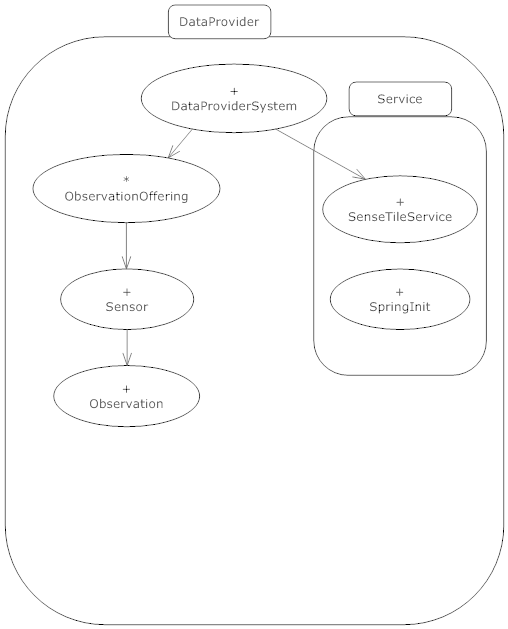
\includegraphics{bon_static_diagam_provider.png}}
\caption{SOS Static Diagram}\label{fig:bon_static_diagam_provider.png}
\end{figure}
The SOS is the main cluster and the Service cluster contains the classes that provide the Web Service interface.

The DataProvider maintains a list of observation offerings provided by the SOS using the ObservationOffering class. When a new sensor type is registered a new ObservationOffering is created. If a DataProvider registers and provides an offering that already exists then just a new Sensor instance is added to the existing ObservationOffering.
 
The Sensor class contains a list of Observations that hold the observations from the DataProvider. The last 50 observations are maintained.

The ObservationService class provides the interface for the DataProducer to update with observations.

The SenseTile Service provides Web Service interface to be used by clients to access the sensor observations.

The SOS specification provides a very rich filtering feature that is too complex for this prototype. The operations are developed in a way to allow the sensor metadata and observations to be retrieved for a specific sensor board. The latest observation or all the stored observations can be retrieved.

\chapter{Implementation}
\section{Overview}
The SenseTile Web Service is written in Java. As described in the high level design there are two components, the DataProducer and the SOS, that are developed to provide this service. The two components are run in separate processes. The communication between the DataProducer and the SOS uses Java RMI. RMI is used due to the SOS and DataProducer
processes are running in the SenseTile Network and communicate over a LAN. This communication protocol has lower overhead than a Web Service so efficient communication between the DataProducer and SOS is achieved. Though it would not be hard to change to use a Web Service as a Java Interface is used to hide the communication mechanism from the main application code. Clients, SOS DataConsumers, access the SOS using a SOAP based Web Service interface. 

The SOS specification describes an implementation using HTTP carry complete operation information encoded in XML including the operations name and parameters. The SenseTile WebService takes a different approach. The operation is defined in the RMI interface and the Web Service Interface while the parameters are encoded in XML thus need parsing.

The following sections describe the DataProducer and SOS implementation.
\section{DataProducer}
The DataProducer, described in section \ref{DataProducerHigh}, accesses the sensor board data and inserts observations into the SOS. Two libraries are used to achieve this: the SensorBoardDriver and the VastSensorMLEngine.

The SensorBoardDriver is described previously in section \ref{SensorBoardDriverSec}. There is also a SensorBoard Simulator library developed by UCS CASL researchers. It produces sensor board packets that can be feed into the DataProvider. This was used during the development of the DataProvider to facilitate testing. 

The VastSensorMLEngine, described in section \ref{VastSensorMLEngineSec}, is used in conjunction with the SenseTile SensorML Model (section \ref{SenseTileModelSec}). The SensorML is parsed by the VastSensorMLEngine into a DOM\footnote{http://www.w3.org/DOM/} tree. To perform the processing it propagates an execute method to the instantiated processes. A ProcessMap.xml file maps SensorML ProcessModel and Component method  URNs  (see section \ref{SMLsection}) to Java classes that provide the implementation of the processing to be performed. 

There is no documentation that I can find for the VastSensorMLEngine. There are some reference implementations of SWE services pointed to from the OGC SWE website \footnote{http://www.ogcnetwork.net/SWE} that provide some information how to use it. The SenseTile SensorML model was not parsed initially by the VastSensorMLEngine. As it opensource the code is available and after a few small changes the model parsed. The VastSensorMLEngine processes the model fine and was very stable during testing.


\section{SOS}
The SOS is the provider of the Web Service interface and is built on Apache Axis2 \footnote{http://ws.apache.org/axis2}. 
Axis2 is described as a "Web Services / SOAP / WSDL engine"  with the Apache Axis2/Java implementation used in this thesis. The Spring framework\footnote{http://www.springsource.org/} was also used. Using these libraries a light Web Service is built to run on the reasonably powerful SenseTile Processor Unit. Axis2 is run standalone here though it can be on with any Servlet engine if a more powerful Web Service is needed.

Developing a Web Service is straight forward with Axis2 and it supports several approaches. The supported POJOs (Plain Old Java Objects) approach was used for the SenseTile Web Service allowing the code to be reused on a different framework if AXIS2 did not work well. Axis2 supports the The Spring framework which is used in the SenseTile WebService for it's dependency injection functionality. A SprinitInit class is needed for Axis2 to load up the Spring framework.

Axis2 provides a tool that automatically generates WSDL from the running Web Service. Another tool allows client side code to be generated from the WSDL easing the development of the Web Service clients.

JAXB \footnote{http://java.sun.com/developer/technicalArticles/WebServices/jaxb} was used for SensorML XML to Java binding in the Web Service. JAXB is able to generate a default binding from the complex SWE schema. Some name collisions were corrected with a JAXB customization file found on the SensorML newsgroups. However the default binding was not fully successful for the System type. It input, output and parameter properties were missing and the inheritance hierarchy did not provide them. A small change was needed to add these properties and then everything worked fine with marshaling and unmarshaling SensorML Systems. 

\chapter{BON to SensorML mapping}
\section{Overview}
In this chapter a BON(see section\ref{BONsec}) to SensorML( see section \ref{SMLsection}) mapping is described. One motivation for this mapping is take advantage of formal software development processes described in \cite{Kiniryref}. This is a verification based process that refines BON to JML and then to Java. Robust software can thus be developed. Another motivation is that it XML is verbose and a more compact description of a SensorML model as facilitated by BON is naturally preferred. Lastly SensorML is complex and it is difficult to develop correct SenorML models based only on using the SensorML XML Schema definition. How a BON specification of SensorML can help here is described later in the chapter.

\section{SensorML BON Specification}
The BON specification of SensorML described is very close conceptually to the SensorML model shown in section \ref{SMLsection}.  The BON SensorML model is shown in figure \ref{fig:bonSensoMLModel}. 
\begin{figure}[h]
\centering
\scalebox{0.65}{\includegraphics{bonSensoMLModel.png}}
\caption{BON SensorML Model}\label{fig:bonSensoMLModel}
\end{figure}
The inheritance heirarhcy is changed slightly with System inheriting from ProcessChain and Component inheriting from ProcessModel. A new abstraction called Port is added. Port contains all the properties of SensorML input, output and parameter as they all have the same properties. A PortType class that ensures legal port types of Input, Output and Parameter is also added to the SenorML BON model.

A BON specification SWE Common data types Count and Quantity are also described along with needed dependent classes. The abstract class DataComponent is the base type for these. There are a many other types but only Count and Quantity are developed as they were the ones used in the SenseTile SensorML model.

The BON specification developed in this thesis does not address the issue of the SensorML metadata and the MetaDataGroup is not specified. This information is for descriptive purposes only and is not used for processing sensor data. BON adds no value here. A different way to add this information to SensorML sensor descriptions is suggested to be used.
AssociationAttributeGroup
SensorML
Member
The complete BON SensorML specification listing can be found in appendix \ref{appenBSMLBONSpec}.

\section{SensorML BON to XML Mapping}
SensorML is essential XML defined by XML Schema with its main purpose being interopeability. Therefore a mapping SensorML BON specification to the SensorML XML is needed. The BON types map closely to SensorML complex types and so a relatively simple scheme is needed.
Effective BON classes map to XML elements. Features in the class map either to attributes of the XML element or a contained XML element. Whether a feature is an attribute is indicated in the class as a comment using @SensorML to make this comment as a mapping instruction. Otherwise an XML element is assumed. The type names of the BON classes and features are the XML element or attribute names. Values. Case of names.

BON SEQUENCE types need a special rule for mapping to SensorML.

Connections rule.

\section{ProcessChain connections problem}
One of the major features of SensorML is the ablity to describe processing chains. The SensorML ProcessChain and System types have a connections property that allows process chaining as decribed in section \ref{SMLref}. Strings are used to describe the connection. An example of this is shown in listing \ref{connectionListing} shows one of the connections from the SenseTile System as described in section \ref{SenseTileModelSec}
\begin{lstlisting}[label=connectionListing,caption=SenseTile System connectionconvertToTemperature]
   <sml:connection name="convertToTemperature">
          <sml:Link>
              <sml:source ref="sensorBoardSystem/outputs/temperatureDNOutput"/>
              <sml:destination ref="convertorSystem/inputs/celciusConvInput"/>
          </sml:Link>
   </sml:connection>

\end{lstlisting}

The source and destination reference strings need to be parsed to find out the inputs and outputs to connect. This is very error prone and the ability to check that connections are correct to a least some degree is desirable. A BON specification can enforce some level of correctness in setting up the connections using preconditions (ensure). The source reference must be either an input of the process chain itself or an output of one of the contained components. In the BON ProcessChain class a feature AddLink checks that Links are legal before adding the Link to the connections feature. This is shown in the BON listing below.

\begin{lstlisting}[basicstyle=\scriptsize,showspaces=false,showstringspaces=false, caption=BON ProcessChaing]  
effective class ProcessChain
     indexing
     about:        "Process formed by chaining sub-processes.";
     title:        "ProcessChain.";
     author:       "Ciaran Palmer.";
     copyright:    "none.";
     organisation: "School of Computer Science and Informatics, UCD.";
     date:         "2010/04/01.";
     version:      "Revision: 1.00.";

     inherit AbstractProcess
     feature
     
     make
       ->componentsIn:AbstractProcess
       require
         componentsIn/=Void;         
       ensure
         delta{components};
         components = componentsIn;
       end
     
     -- Collection of subprocesses that can be chained using connections      
     components:SEQUENCE[AbstractProcess]
     
     -- Links between processes
     connections:SEQUENCE[Link]
     
     -- Add a link with check that Link is legal
     AddLink
        ->linkIn:Link
      require
          linkIn /= Void;

           -- check Link source is legal
          (exists i:INTEGER such_that linkIn.source = Current.inputs[i]) or\
          \(exists i:INTEGER and j:INTEGER such_that linkIn.source =\
          \components[j].outputs[i]);

          -- check Link destination is legal
          (exists i:INTEGER such_that linkIn.destination = Current.outputs[i]) or\
          \(exists i:INTEGER and j:INTEGER such_that linkIn.destination =\
          \components[j].inputs[i]);

        ensure
           delta{connections};
          (exists i:INTEGER such_that connections[i] linkIn);
      
      invariant
        components /= Void;
        
  end --ProcessChain
 \end{lstlisting}


\section{SenseTile Thermistor BON SensorML Specification }
Thermistor can be generated by the following BON class.

\chapter{Results}

A  SensorML Model of the UCD CASL SenseTile sensor system was developed to evaluate SensorML. The SenseTile Sensor Board and Thermistor sensor were the focus of the model. Appendix \ref{appenA} shows the full SensorML SenseTile model developed.

A lightweight Web Service was developed to explore the use of SensorML and SOS specifications in sensor systems. The Web Service is implemented in Java and is built on AXIS2.0, the Spring framework, the VASTSensorMLEngine and the UCD CASL SensorBoardDriver. It was tested against SenseTile SensorBoard Simulator classes using a basic test client.

A BON specification was developed for the core SensorML types and the SWE Common Data types used in the SenseTile SensorML model. The BON specification is included in appendix \ref{appenB} A BON to SensorML XML encoding mapping is also developed and is included in appendix \ref{appenC}.

\chapter{ Conclusions and Future Work}
\subsection{Conclusions}
This project analyses the role of the SensorML and SOS specifications in sensor systems. The UCD CASL SenseTile System is used as a case study for the use of these specifications with a SensorML model of the SenseTile system developed to evaluate SensorML. A SenseTile Web Service prototype is developed to evaluate the SOS specification which uses SensorML to provide sensor descriptions to clients. 

SensorML provides a simple functional model of sensors in terms of an intuitive process concept. A process transforms sensor inputs to outputs as modeled by the SensorML AbstractProcess type. SensorML provides a process chaining capability to break up complex processing into smaller more manageable steps. There is also a rich set of data types to describe the sensor data. Due to the simple yet flexible model and the rich set of data types is is hard to see any sensor or sensor system that could not be described by SensorML.
This is part of its goal to be a standard of interoperability of sensor system. The Sensor XML encoding provided furthers this goal. SensorML also provides a good level of metadata types to assist with a human understanding of the capabilities of the sensor system.

SensorML provides good support for the reliable processing of sensor data. The data types have properties that can reference definitions to precisely describe their meaning or give an indication of the quality of the data.  The accuracy of the sensor can be modeled and can be provided to processes using parameters to get a more accurate output from the process.

It could model the SenseTile system well at this functional level. 
SensorML is relatively intuitive but it is difficult to know if one has developed a "good" SensorML model. There are examples and tutorials to help. 

SensorML is not intended to provide the framework for encoding the actual

SensorML is defined by a complex set of XML Schema. Achieving a Java to XML binding was difficult based on these schema. JIBX\footnote{http://jibx.sourceforge.net/} would not generate a default XML binding. JAXB could with some help. There are many layers of abstraction in these XML Schema. This reflects the that the specifications cover a very wide range of needs of a senor system. 

The Vast Lib seems to be the reference implementation of a SensorML processing framework. There was little or no documentation that I could find on this and examples of it's use needed some research. It would be better if a working example could be provided with the framework and also some basic documentation. The Vast code needed to be slightly modified to parse the SenseTile model files though they passed a validation check\footnote{http://vast.uah.edu/SensorMLforms/validate.jsp} provided by the Vast group. After these updates allowed the parsing to finish the code was indeed very stable and never crashed except when there were mistakes in the SenseTile SensorML XML files.

The SWE SOS specification describes the operations for accessing sensor observations and it's concepts were used to develop the SenseTile Web Service. It uses SensorML provide sensor metadata to clients and the O\&M specification to encode observations.
Implement all functionality would be difficult. Maybe too heavy for SenseTile System. Simple querires. Or better a push system to send the data to the client as it is generated could be a better approach here.

The SOS specification is complex. If there no need for interoperability or a rich filtering ability of sensor data provided by the SOS operations then it is better to go with some other simpler approach.  This approach could be use standard Web Services and use SensorML for sensor descriptions.

SOS Scalable hierarcy of instances.

SWE not fully web services as W3C might define. Not SOAP. HTTP envelope
flexible. There seems to be work ongoing to change this to a more industry standard view of Web Services with the use of WSDL/SOAP. I could not find this as part of current OGC SWE framework.
what has been achieve

SOS on the Processor Board. Is this right? RMI only useful if SenseTile Network is a lan.

BON

Working in XML is error prone. SensorML connections type was a good example of where a graphical tool or another language, like BON,  that can be parsed should be used to check the connections. Running the model through the VastSensorMLEngine without a crash was only way other than by eye to see that the connections were set up correctly. 


\subsection{Future Work}
SensorML sensor accuracy.
Complete BON mapping and parser.
Streaming the data. See SWE Architecture dpcument for a description of one approach.
Other technology approaches such as . Other ways such a XQUERY? XML techs?

\newpage
\begin{thebibliography}{99}
\bibitem{OSWAref} Chu, Kobialka,  Durnota, and  Buyya, Open Sensor Web Architecture: Core Services
\bibitem{SMLref}Open Geospatial Consortium Inc., OpenGIS Sensor Model Language (SensorML) Implementation Specification, 2007
\bibitem{SOSref}Open Geospatial Consortium Inc.,  Sensor Observation Service, 2007
\bibitem{Kiniryref}Kim Waldén and Jean-Marc Nerson , "Seamless Object-Oriented Software Architecture", 1995
\bibitem{OMref}Open Geospatial Consortium Inc., Observations and Measurements – Part 1 - Observation schema, 2007
\bibitem{SWEArchref}Open Geospatial Consortium Inc., OGC Sensor Web Enablement Architecture, 2008
\bibitem{SMLTutorialref}Open Geospatial Consortium Inc., Using SensorML to describe a
Complete Weather Station , 2006
\bibitem{ProcessTutorialref}Open Geospatial Consortium Inc.,
\bibitem{OGCcatref}Open Geospatial Consortium Inc., OpenGIS® Catalogue Services Specification, 2007
\bibitem{Meyerref}Bertrand Meyer., "Object-Oriented Software Construction", 1997

\end{thebibliography}



\appendix
\chapter{Appendix: SenseTile SensorML Model}\label{appenA}
\section{SenseTile SensorML System}
\section{SenseTile SensorML SensorBoardSystem}
\section{SenseTile SensorML ConvetorSystem}
\section{SenseTile SensorML Thermistor}
\lstinputlisting{Thermistor.xml}
\section{SenseTile SensorML CelciusConvertor}


\chapter{Appendix: BON to SensorML Mapping}\label{appenB}
\section {SensorML BON Specifcation}\label{appenBSMLBONSpec}

\lstset{basicstyle=\scriptsize,showspaces=false,showstringspaces=false}
\lstinputlisting{SensorML_formal.bon}
\section {BON to SensorML mapping tables} \label{appenBSMLBONTables}
\lstset{frame=none}
\begin{table}[!th]
\centering
\begin{tabular}{|l|l|}
\hline
BON features & SensorML XML tags\\
\hline
   deferred class AbstractProcess  & not mapped\\
\hline     
     inputs:SEQUENCE[Input] & \begin{lstlisting}
<sml:inputs><sml:inputlist>
SEQUENCE[Input]
<\sml:InputList><\sml:inputs>\end{lstlisting}\\

\hline 
     outputs:SEQUENCE[Output] & \begin{lstlisting}
<sml:outputs><sml:outputlist>
SEQUENCE[Input]
<\sml:outputList><\sml:outputs>\end{lstlisting}\\
\hline
     parameters:SEQUENCE[Parameter] & \begin{lstlisting}
<sml:parameters><sml:parametertlist>
SEQUENCE[Input]
<\sml:outputList><\sml:outputs>\end{lstlisting}\\

\hline                 
     metaDataGroup:MetaDataGroup &  \begin{lstlisting}
<\sml:metaDataGroup><\sml:metaDataGroup>\end{lstlisting}\\
 \hline    

\end{tabular}
\caption{BON to SensorML AbstractProcess Mapping table}\label{table:bon_sml_example}
\label{ex:table}
\end{table}


\begin{table}[!th]
\centering
\begin{tabular}{|l|l|}
\hline
BON features & SensorML XML tags\\
\hline
   deferred class System  & not mapped\\
\hline     
     inputs:SEQUENCE[Input] & \begin{lstlisting}
<sml:inputs><sml:inputlist>
SEQUENCE[Input]
<\sml:InputList><\sml:inputs>\end{lstlisting}\\

\hline 
     outputs:SEQUENCE[Output] & \begin{lstlisting}
<sml:outputs><sml:outputlist>
SEQUENCE[Input]
<\sml:outputList><\sml:outputs>\end{lstlisting}\\
\hline
     parameters:SEQUENCE[Parameter] & \begin{lstlisting}
<sml:parameters><sml:parametertlist>
SEQUENCE[Input]
<\sml:outputList><\sml:outputs>\end{lstlisting}\\

\hline                 
     metaDataGroup:MetaDataGroup &  \begin{lstlisting}
<\sml:metaDataGroup><\sml:metaDataGroup>\end{lstlisting}\\
 \hline    

\end{tabular}
\caption{BON to SensorML AbstractProcess Mapping table}\label{table:bon_sml_example}
\label{ex:table}
\end{table}

\begin{table}[!th]
\centering
\begin{tabular}{|l|l|}
\hline
BON features & SensorML XML tags\\
\hline
   deferred class C  & not mapped\\
\hline     
     inputs:SEQUENCE[Input] & \begin{lstlisting}
<sml:inputs><sml:inputlist>
SEQUENCE[Input]
<\sml:InputList><\sml:inputs>\end{lstlisting}\\

\hline 
     outputs:SEQUENCE[Output] & \begin{lstlisting}
<sml:outputs><sml:outputlist>
SEQUENCE[Input]
<\sml:outputList><\sml:outputs>\end{lstlisting}\\
\hline
     parameters:SEQUENCE[Parameter] & \begin{lstlisting}
<sml:parameters><sml:parametertlist>
SEQUENCE[Input]
<\sml:outputList><\sml:outputs>\end{lstlisting}\\

\hline                 
     metaDataGroup:MetaDataGroup &  \begin{lstlisting}
<\sml:metaDataGroup><\sml:metaDataGroup>\end{lstlisting}\\
 \hline    

\end{tabular}
\caption{BON to SensorML AbstractProcess Mapping table}\label{table:bon_sml_example}
\label{ex:table}
\end{table}

\begin{table}[!th]
\centering
\begin{tabular}{|l|l|}
\hline
BON features & SensorML XML tags\\
\hline
   deferred class Link  & not mapped\\
\hline     
     inputs:SEQUENCE[Input] & \begin{lstlisting}
<sml:inputs><sml:inputlist>
SEQUENCE[Input]
<\sml:InputList><\sml:inputs>\end{lstlisting}\\

\hline 
     outputs:SEQUENCE[Output] & \begin{lstlisting}
<sml:outputs><sml:outputlist>
SEQUENCE[Input]
<\sml:outputList><\sml:outputs>\end{lstlisting}\\
\hline
     parameters:SEQUENCE[Parameter] & \begin{lstlisting}
<sml:parameters><sml:parametertlist>
SEQUENCE[Input]
<\sml:outputList><\sml:outputs>\end{lstlisting}\\

\hline                 
     metaDataGroup:MetaDataGroup &  \begin{lstlisting}
<\sml:metaDataGroup><\sml:metaDataGroup>\end{lstlisting}\\
 \hline    

\end{tabular}
\caption{BON to SensorML AbstractProcess Mapping table}\label{table:bon_sml_example}
\label{ex:table}
\end{table}

\begin{table}[!th]
\centering
\begin{tabular}{|l|l|}
\hline
BON features & SensorML XML tags\\
\hline
   deferred class ProcessChain  & not mapped\\
\hline     
     inputs:SEQUENCE[Input] & \begin{lstlisting}
<sml:inputs><sml:inputlist>
SEQUENCE[Input]
<\sml:InputList><\sml:inputs>\end{lstlisting}\\

\hline 
     outputs:SEQUENCE[Output] & \begin{lstlisting}
<sml:outputs><sml:outputlist>
SEQUENCE[Input]
<\sml:outputList><\sml:outputs>\end{lstlisting}\\
\hline
     parameters:SEQUENCE[Parameter] & \begin{lstlisting}
<sml:parameters><sml:parametertlist>
SEQUENCE[Input]
<\sml:outputList><\sml:outputs>\end{lstlisting}\\

\hline                 
     metaDataGroup:MetaDataGroup &  \begin{lstlisting}
<\sml:metaDataGroup><\sml:metaDataGroup>\end{lstlisting}\\
 \hline    

\end{tabular}
\caption{BON to SensorML AbstractProcess Mapping table}\label{table:bon_sml_example}
\label{ex:table}
\end{table}

\begin{table}[!th]
\centering
\begin{tabular}{|l|l|}
\hline
BON features & SensorML XML tags\\
\hline
   deferred class ProcessModel  & not mapped\\
\hline     
     inputs:SEQUENCE[Input] & \begin{lstlisting}
<sml:inputs><sml:inputlist>
SEQUENCE[Input]
<\sml:InputList><\sml:inputs>\end{lstlisting}\\

\hline 
     outputs:SEQUENCE[Output] & \begin{lstlisting}
<sml:outputs><sml:outputlist>
SEQUENCE[Input]
<\sml:outputList><\sml:outputs>\end{lstlisting}\\
\hline
     parameters:SEQUENCE[Parameter] & \begin{lstlisting}
<sml:parameters><sml:parametertlist>
SEQUENCE[Input]
<\sml:outputList><\sml:outputs>\end{lstlisting}\\

\hline                 
     metaDataGroup:MetaDataGroup &  \begin{lstlisting}
<\sml:metaDataGroup><\sml:metaDataGroup>\end{lstlisting}\\
 \hline    

\end{tabular}
\caption{BON to SensorML AbstractProcess Mapping table}\label{table:bon_sml_example}
\label{ex:table}
\end{table}

\begin{table}[!th]
\centering
\begin{tabular}{|l|l|}
\hline
BON features & SensorML XML tags\\
\hline
   deferred class Port  & not mapped\\
\hline     
     inputs:SEQUENCE[Input] & \begin{lstlisting}
<sml:inputs><sml:inputlist>
SEQUENCE[Input]
<\sml:InputList><\sml:inputs>\end{lstlisting}\\

\hline 
     outputs:SEQUENCE[Output] & \begin{lstlisting}
<sml:outputs><sml:outputlist>
SEQUENCE[Input]
<\sml:outputList><\sml:outputs>\end{lstlisting}\\
\hline
     parameters:SEQUENCE[Parameter] & \begin{lstlisting}
<sml:parameters><sml:parametertlist>
SEQUENCE[Input]
<\sml:outputList><\sml:outputs>\end{lstlisting}\\

\hline                 
     metaDataGroup:MetaDataGroup &  \begin{lstlisting}
<\sml:metaDataGroup><\sml:metaDataGroup>\end{lstlisting}\\
 \hline    

\end{tabular}
\caption{BON to SensorML AbstractProcess Mapping table}\label{table:bon_sml_example}
\label{ex:table}
\end{table}

\begin{table}[!th]
\centering
\begin{tabular}{|l|l|}
\hline
BON features & SensorML XML tags\\
\hline
   deferred class Quantity  & not mapped\\
\hline     
     inputs:SEQUENCE[Input] & \begin{lstlisting}
<sml:inputs><sml:inputlist>
SEQUENCE[Input]
<\sml:InputList><\sml:inputs>\end{lstlisting}\\

\hline 
     outputs:SEQUENCE[Output] & \begin{lstlisting}
<sml:outputs><sml:outputlist>
SEQUENCE[Input]
<\sml:outputList><\sml:outputs>\end{lstlisting}\\
\hline
     parameters:SEQUENCE[Parameter] & \begin{lstlisting}
<sml:parameters><sml:parametertlist>
SEQUENCE[Input]
<\sml:outputList><\sml:outputs>\end{lstlisting}\\

\hline                 
     metaDataGroup:MetaDataGroup &  \begin{lstlisting}
<\sml:metaDataGroup><\sml:metaDataGroup>\end{lstlisting}\\
 \hline    

\end{tabular}
\caption{BON to SensorML AbstractProcess Mapping table}\label{table:bon_sml_example}
\label{ex:table}
\end{table}

\begin{table}[!th]
\centering
\begin{tabular}{|l|l|}
\hline
BON features & SensorML XML tags\\
\hline
   deferred class Count  & not mapped\\
\hline     
     inputs:SEQUENCE[Input] & \begin{lstlisting}
<sml:inputs><sml:inputlist>
SEQUENCE[Input]
<\sml:InputList><\sml:inputs>\end{lstlisting}\\

\hline 
     outputs:SEQUENCE[Output] & \begin{lstlisting}
<sml:outputs><sml:outputlist>
SEQUENCE[Input]
<\sml:outputList><\sml:outputs>\end{lstlisting}\\
\hline
     parameters:SEQUENCE[Parameter] & \begin{lstlisting}
<sml:parameters><sml:parametertlist>
SEQUENCE[Input]
<\sml:outputList><\sml:outputs>\end{lstlisting}\\

\hline                 
     metaDataGroup:MetaDataGroup &  \begin{lstlisting}
<\sml:metaDataGroup><\sml:metaDataGroup>\end{lstlisting}\\
 \hline    

\end{tabular}
\caption{BON to SensorML AbstractProcess Mapping table}\label{table:bon_sml_example}
\label{ex:table}
\end{table}


\label{endpage}
\end{document}

\end{article}
